% !TEX root = Bachelorarbeit_Paul_Zilewitsch.tex
\section{Service Desk nach ITIL v3}

\subsection{Begriffsabgrenzung}
\noindent Für die Klärung des Begriffs \enquote{Service Desk} ist es sinnvoll, sich auf die Information Technology Infrastructure Library - kurz ITIL - zu beziehen.
ITIL ist zwar keine Norm, die in der IT-Branche eingehalten werden muss, dennoch bezieht man sich im IT-Service Management vorrangig auf ITIL.
Bereits 1989 wurde die Central Computer and Telecommunication Agency (CCTA) von der britischen Regierung beauftragt, Geschäftsprozesse und ihre Abhängigkeiten zu beschreiben und schriftlich festzuhalten.\footnote{Vgl. \citeauthor{Olbrich} (\citeyear{Olbrich}), S. 1.}
Ziel war es, Abläufe in der Unternehmenswelt darzustellen und dadurch die IT-Betriebskosten zu reduzieren. Im Laufe der Jahre wurden die ersten Ausarbeitungen überarbeitet und ergänzt. Die ITIL Edition 2011 ist die derzeitig neuste Fassung und stellt ein Update der 2007 veröffentlichten Version ITIL v3 dar.\footnote{Website: \citeauthor{Andenmatten} (abgerufen am: 10.05.2016)}
Auch bestimmte Normen leiten sich aus dem ITIL-Rahmenkonzept ab. Der internationale Standard ISO/IEC 20000 beispielsweise basiert auf der Version ITIL v2 und definiert die Minimalanforderungen des IT-Service-Managements für Organisationen.\footnote{Vgl. \citeauthor{Buchsein} (\citeyear{Buchsein}), S. 5ff.}
ITIL kann deshalb als "Quasi-Standard" gesehen werden. Es ist ein  Best-Practice Leitfaden, der beschreibt "Was zu tun ist, aber nicht wie". Das macht deutlich, dass ITIL durchaus Handlungs -und Interpretationsspielraum zulässt, aber dennoch in einem vorher definierten Rahmen greifbar sein muss. Beschrieben wird ITIL v3 in fünf Büchern, auf die später noch eingegangen wird:

\begin{itemize}
\item Service Strategy
\item Service Design
\item Service Transition
\item Service Operation
\item Continual Service Improvement
\end{itemize}

\noindent
ITIL kann als Framework gesehen werden, mit dem Abläufe im Bereich IT Service beschrieben werden können. Genauer gesagt, spricht man von IT Services Management, kurz ITSM. Hier werden alle Methoden erläutert, die nötig sind, um die bestmögliche Unterstützung von Geschäftsprozessen durch die IT-Organisation zu erreichen.\footnote{Vgl. \citeauthor{Ebel} (\citeyear{Ebel}), S. 27ff.} In ITIL ist der Prozess definiert als ein \enquote{Satz von in Wechselbeziehung oder Wechselwirkung stehenden Tätigkeiten (und Mitteln), die Eingaben in Ergebnisse umwandelt.}\footnote{Vgl. \citeauthor{ISO9000} (\citeyear{ISO9000}), S. 23.} Zu den Mitteln können Personal, Einrichtungen und Anlagen, Technologie und Methodologie gehören. Eingaben für einen Prozess sind üblicherweise  Ergebnisse anderer Prozesse.

\noindent
Jeder IT Service Management-Prozess hat eine charakteristische Zielrichtung und wird durch Funktionen unterstützt. Eine Funktion besteht aus einer Gruppe von Personen und deren Werkzeugen, die dafür verwendet werden, ein oder mehrere Prozesse oder Aktivitäten zu stützen.\footnote{Vgl. \citeauthor{Cannon} (\citeyear{Cannon}), S. 233.} Außerdem bewirkt das Zusammenspiel verschiedener IT Service Management-Prozesse, dass dem Kunden die notwendigen IT Services zur wirkungsvollen Unterstützung seiner Geschäftsprozesse geliefert werden. Der Service Lifecycle in Abbildung~\ref{fig:ITIL_Lebenyzyklus} veranschaulicht genau diese Kernprozesse und Kernfunktionen, die ein IT-Prozess während seiner gesamten Lebensdauer besitzt. Die einzelnen Teilbereiche decken sich mit den zuvor aufgeführten Büchern von ITIL v3.\footnote{Vgl. \citeauthor{Ebel} (\citeyear{Ebel}), S. 27ff.}

\begin{figure}[h!]
\centering
	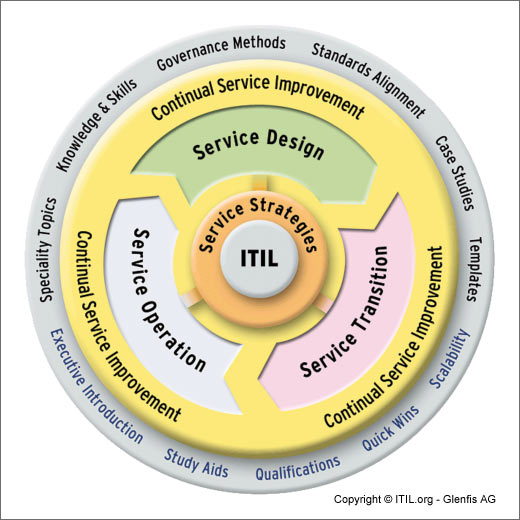
\includegraphics[width=0.50\textwidth]{Abbildungen/ITIL_Lebenszyklus}
	\caption[ITIL Service Lifecycle]{ITIL Service Lifecycle, Quelle: \url{http://os.itil.org/osMedia/site/t1 
	media/JPEG/01_itil_imap.jpg}}
	\label{fig:ITIL_Lebenyzyklus}
\end{figure}

\noindent
Es ist nicht notwendig, auf alle Teilbereiche einzugehen. Der Service Desk ist nämlich Bestandteil der Service Operation und somit die richtige Anlaufstelle für die Begriffsklärung. \newline \enquote{Service Operation beschreibt den Abschnitt des Lebenszyklus, der von den Kunden primär wahrgenommen wird.}\footnote{\citeauthor{Ebel} (\citeyear{Ebel}), S. 439.} In der Service Operations-Phase werden die Prozesse und Funktionen beschrieben, die einen stabilen  und bestmöglichen IT Service garantieren sollen. Bei dieser Verbindung von IT Organisation und Kunde wird besonders auf den Kunden eingegangen. Der Service Desk ist hierbei \enquote{die zentrale Anlaufstelle, der Single Point of Contact (SPoC) zwischen Anwender und der IT-Organisation}.\footnote{\citeauthor{Ebel} (\citeyear{Ebel}), S. 439.} Wie der Name schon verrät, kommt der Anwender nur über diese Schnittstelle in Kontakt mit der IT. Hier werden Meldungen der Anwender üblicherweise erfasst, kategorisiert und eingetragen. Der Service Desk ist nicht nur eine Kommunikationsunterstützung, sondern bietet gleichzeitig eine Auskunft für bereits bekannte Probleme. Dadurch kann bei häufig auftretenden Service-Unterbrechungen schneller gehandelt werden. Auch Supportanfragen, Beschwerden, Verbesserungsvorschläge oder Änderungswünsche können in den Service Desk eingetragen werden. Der Service Desk fungiert dadurch als sogenannter \enquote{Single Point of Contact}. Die nachfolgende Abbildung macht deutlich, dass der Kunde (Anwender) eine einzige Anlaufstelle hat, um seine Anliegen dem Support mitzuteilen. 

\begin{figure}[h!]
\centering
	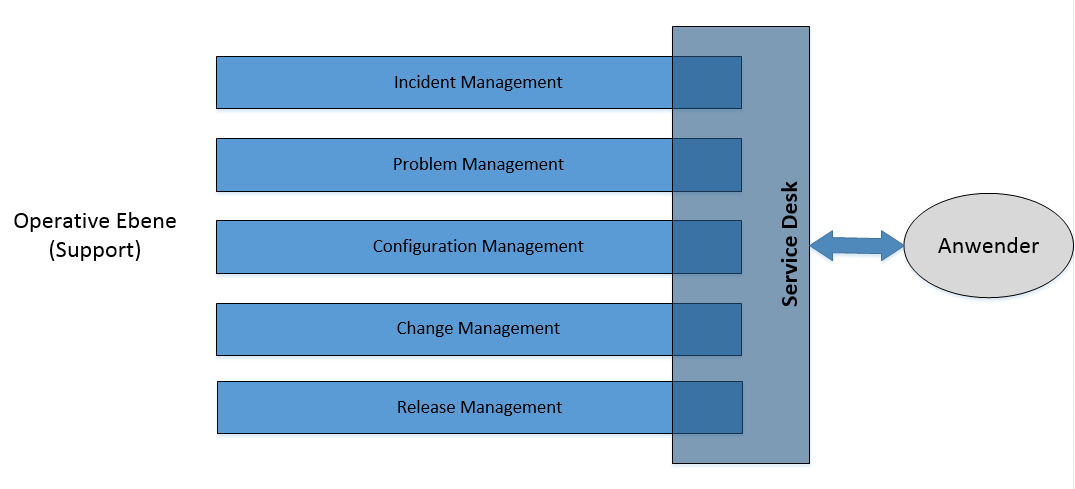
\includegraphics[width=0.70\textwidth]{Abbildungen/SPOC_3.png}
	\caption[Single Point of Contact]{Single Point of Contact, Quelle:http://edoc.hu-berlin.de/
	conferences/dfn2006/fischlin-roger-105/PDF/fischlin.pdf}
	\label{fig:ITIL_Single_Point_of_Contact}
\end{figure}

\noindent
Der Support kann die Meldungen der Anwender nun den entsprechenden Managementbereichen zuordnen. Eine Störmeldung von einem technischen Gerät würde beispielsweise zum Incident Management gehören. Ein Feature-Wunsch ist eher dem Teilbereich Change Management einzuordnen. Der Single Point of Contact  erleichtert so die Kommunikation zwischen dem Anwender und dem Support.\footnote{Vgl. \citeauthor{Ebel} (\citeyear{Ebel}), S. 65 ff.}\\ 


\subsection{Unterschied zu Help Desk}
\noindent
Bei der Begriffsabgrenzung zwischen Help Desk und Service Desk ist Vorsicht geboten. In mehreren Quellen ist zu finden, dass Help Desk (auch User-Help-Desk) lediglich ein veralteter Begriff für den Service Desk sei.\footnote{Vgl. \citeauthor{Buchsein} (\citeyear{Buchsein}), S. 26.}\footnote{Vgl. \citeauthor{Meier} (\citeyear{Meier}), S. 26.} Im Internet heißt es beispielsweise auf Wikipedia: \enquote{Die Artikel Helpdesk und Servicedesk überschneiden sich thematisch.}\footnote{Website: \citeauthor{WikiServiceDesk} (abgerufen am: 24.05.2016)} In anderen Literaturquellen tritt der Begriff Help Desk erst gar nicht auf oder wird dem Service Desk gleichgesetzt.\footnote{Vgl. \citeauthor{Olbrich} (\citeyear{Olbrich}), S. 19.} Im Zweifelsfall sollte man sich direkt auf das Buch ITIL Service Operation beziehen. In dem heißt es übersetzt unter dem Stichwort Help Desk:
\enquote{Eine Anlaufstelle für Anwender, um Incidents zu erfassen. Ein Help Desk ist in der
Regel eher technisch orientiert als ein Service Desk und stellt keinen Single Point
of Contact für die gesamte Interaktion bereit. Der Begriff 'Help Desk' wird häufig
auch als Synonym für Service Desk verwendet.}\footnote{\citeauthor{Cannon} (\citeyear{Cannon}), S. 233. Übersetzung entnommen aus: Ebel, N. (2008) S. 699.} \newline
In den weiteren Ausführungen gilt deshalb der Help Desk als Synonym für den Service Desk.

\newpage


\subsection{Aufgaben eines Service Desk}
\noindent
Im Folgenden sollen die wichtigsten Aufgaben eines Service Desk aus Sicht der ITIL v3 betrachtet werden. Hierfür wird zunächst stichpunktartig die Kernaussage festgehalten, um sie anschließend zu erläutern. Dabei beziehen sich die Kernaussagen auf die Ausarbeitung Olbrichs aus \enquote{ITIL Kompakt und verständlich}\footnote{\citeauthor{Olbrich} (\citeyear{Olbrich}), S. 19f.}
und sind eine leicht abgewandelte Form vom ITIL v3 Band Service Operation.\footnote{Vgl. \citeauthor{Cannon} (\citeyear{Cannon}), S. 110.}

\begin{itemize}
\item \enquote{Einheitlichen, zentralen Kommunikationsschnittstelle (SPoC) mit konkreten Ansprechpartner}
\end{itemize}
\noindent
Der Kunde hat mehrere Möglichkeiten, den Support zu kontaktieren. Schreibt der Kunde eine E-Mail an den Support, könnte diese ausgewertet und im Service Desk eingetragen werden. Ebenso könnte er selbst einen Eintrag über ein Web-Frontend erstellen. Oder aber der Support erstellt einen solchen Eintrag im Service Desk, wenn der Kunde zum Telefon greift. Es ist jedoch Voraussetzung, dass eine einheitliche und zentrale Kommunikationsschnittstelle bereitgestellt wird.


\begin{itemize}
\item \enquote{Aufnahme, Dokumentation und Auswertung aller Vorfälle}
\end{itemize}
\noindent
Wenn alle Vorfälle ordnungsgemäß aufgenommen und dokumentiert wurden, kann schneller reagiert werden, wenn sich ein Problem wiederholt. Dass alle Vorfälle auch ausgewertet werden sollten, ist verständlich und kann eventuell dazu beitragen, Folgeprobleme frühzeitig zu erkennen.

\begin{itemize}
\item \enquote{Überwachung, Nachverfolgung und Eskalation von laufenden
Supportvorgängen. Frühzeitiges Erkennen von
Bedürfnissen und Problemsituationen}
\end{itemize}
\noindent
Wie im Punkt zuvor erwähnt, können Probleme frühzeitig erkannt werden, indem Vorfälle genauestens ausgewertet werden. Das ist aber längst nicht die einzige Möglichkeit, Bedürfnisse der Kunden zu erkennen. Gute Mittel für vorausschauende Handlungen sind  bspw. Monitoring-Systeme oder Log-Files. Sie liefern technische Informationen, die - nach einer Auswertung - Aufschluss über die aktuelle Lage des Kunden geben und in den Service Desk integriert werden könnten. Nach ITIL v3 gibt es zwei Arten von Eskalation. Die funktionale Eskalation, bei der ein besonders schweres Problem oder die vergangene Zeit ein Auslöser wie die Eskalation eines Incidents ist. Im Gegensatz dazu ist bei hierarchische Eskalation eine Weiterleitung des Problems an die nächst höhere Eskalationshierarchie vorgesehen. Sollte beispielsweise ein Problem im Service Desk längere Zeit nicht bearbeitet und somit kein Fortschritt erzielt werden, eskaliert das Problem und wird entsprechend weitergeleitet\footnote{Vgl. \citeauthor{ITILBuch} (\citeyear{Victor}), S. 80f.}\footnote{Vgl. \citeauthor{Victor} (\citeyear{Victor}), S. 26ff.}


\begin{itemize}
\item \enquote{Überprüfung der Einhaltung des Dienstleistungsgegenstands
anhand von Service-Level-Agreements}
\end{itemize}
\noindent
Mithilfe des Service Desks kann kontrolliert werden, ob die vereinbarten Leistungen zwischen Auftraggeber und Beauftragten eingehalten wurden, wenn alle Vorfälle dokumentiert wurden.

\begin{itemize}
\item \enquote{Reporting – Beauskunftung gegenüber den Usern (Kunden)
und dem Management. Informationen über den aktuellen
Status von Vorgängen, geplanten Änderungen und
verschiedenen Nutzungsmöglichkeiten}
\end{itemize}
\noindent
Der Service Desk dient außerdem dazu, stets mit dem Kunden im Kontakt zu stehen. So können Informationen an den Kunden weitergeleitet oder auf der anderen Seite aktuelle Vorgänge, Status etc. des Kunden verfolgt und analysiert werden. 

\begin{itemize}
\item \enquote{Überprüfen der Kundenzufriedenheit, Stärkung der Kundenbeziehung.
Kontaktpflege. Aufspüren neuer Geschäftschancen}
\end{itemize}
\noindent
Nicht zuletzt kann der Service Desk auch als Instrument für einen ständigen Kontakt zum Kunden eingesetzt werden. Der Kunde hat dadurch den Eindruck, permanent mit der Support und somit der Firma verbunden zu sein. Das kann das Verhältnis zum Kunden stärken oder gar neue Geschäftsmöglichkeiten eröffnen.\\\\



\subsection{Nachteile ohne Servie Desk}
\noindent
Die vielseitigen Aufgaben eines Service Desk machen deutlich, welche Nachteile ein nicht vorhandener Service Desk für ein Unternehmen haben kann. Benutzer wissen bei Problemfällen nicht sofort, wer für die Bearbeitung des Vorfalls zuständig ist. Auch ist der Melder beispielsweise für eine Störmeldung nicht sofort identifizierbar. Rückfragen sind daher schwer möglich und die gesamte Bearbeitung des Problems verzögert sich stark.\\

\noindent 
Bei der Erfassung von Vorfallen sind im Service Desk bestimmte Informationen nötig, die normalerweise über ein Formular o.ä. erfasst werden. Wenn der Service Desk - und damit auch ein Formular zu Erfassung - komplett fehlt, kann es zu unvollständigen Vorfallbeschreibungen kommen. Auch hier wird der Prozess für die Problembehandlung verlangsamt.\\

\noindent
Probleme, die häufig auftreten, werden nur teilweise bis gar nicht dokumentiert. Dadurch werden immer wieder neue Lösungsansätze gesucht, ohne auf bereits vorhandene und bewährte Lösungen zurückzugreifen. Eine Wissensdatenbank ist daher unmöglich.\\

\noindent
Das Anschaffen einer Service Desk-Lösung sowie die zugehörigen Schulungsausgaben sind natürlich mit Kosten verbunden, doch ein effektives Vorgehen beim Lösen eines Vorfalls mittels des Service Desks kann die Gesamtkosten reduzieren. Demzufolge würde ein gut implementierter Service Desk dazu beitragen, die Kosten insgesamt zu senken.\footnote{Vgl. \citeauthor{Olbrich} (\citeyear{Olbrich}), S. 26f.}\\

\noindent
Unter bestimmten Voraussetzungen ist es möglich, dass ein Kunde direkt mit dem Fachpersonal - beispielsweise aus der Entwicklungsabteilung - kommuniziert, anstatt mit einem Supportmitarbeiter. Das geschieht, wenn keine Filterung der eingetroffenen Probleme vorgenommen wird. Ein Entwickler könnte somit einem fragenden Kunden gegenüberstehen, dessen Problem eher in den Bereich Release Management einzuordnen ist. Ein Supportmitarbeiter wäre in diesem Fall der bessere Gesprächspartner für den Kunden.\\

\noindent
Der Kunde hat beim Fehlen eines Service Desk keinen Single Point of Contact mehr und könnte möglicherweise nicht wissen, an wen er sich bei Problemen zu wenden hat. Es fehlt ein wichtiger Kommunikationsweg, der nicht ohne weiteres ersetzt werden kann. Dadurch könnte auch die Beziehung zwischen dem Unternehmen und dem Kunden leiden.\\\\



\noindent
In diesem Punkt wurden die begrifflichen Grundlagen für das weitere Vorgehen gelegt. Es wurde deutlich gemacht, welche Aufgaben ein Service Desk hat und somit auch, wie wichtig er für die Kommunikationsstruktur eines Unternehmens sein kann. Nicht nur der Kontakt zum Kunden kann durch den Service Desk verbessert werden, auch das Protokollieren und Lösen von Problemen innerhalb einer Firma ist mit dem Service Desk besser zu bewältigen.\newline









   


 
